\begin{figure}[h]
 \center
 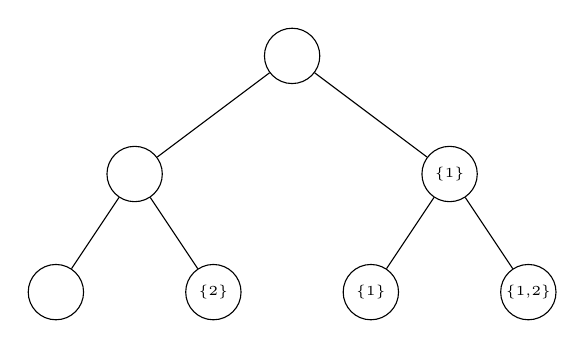
\begin{tikzpicture}[level/.style={sibling distance=40mm/#1}]
 \node [circle,draw,minimum size=20pt,inner sep=0pt] (z){$\varnothing$} 
  child {node [circle,draw,minimum size=20pt,inner sep=0pt] (a) {$\varnothing$}
   child {node [circle,draw,minimum size=20pt,inner sep=0pt] (b) {$\varnothing$}}
   child {node [circle,draw,minimum size=20pt,inner sep=0pt] (c) {$\scriptscriptstyle \{2\}$} }
  }
  child {node [circle,draw,minimum size=20pt,inner sep=0pt] (d) {$\scriptscriptstyle\{1\}$}
   child {node [circle,draw,minimum size=20pt,inner sep=0pt] (e) {$\scriptscriptstyle\{1\}$} }
   child {node [circle,draw,minimum size=20pt,inner sep=0pt] (f) {$\scriptscriptstyle\{1,2\}$} }
  };
 \end{tikzpicture}
 \caption{背包问题的搜索树}
 \label{fig:knapsack_tree}
\end{figure}
